\documentclass[aspectratio=169,11pt]{beamer}
\usefonttheme{professionalfonts}
\usepackage{fontspec}
\defaultfontfeatures{Ligatures=TeX}
\usepackage{polyglossia}
\setdefaultlanguage{russian}
\setotherlanguage{english}
\usepackage{amsmath,amssymb}
\usepackage{unicode-math}
\setmainfont{Arial}\setsansfont{Arial}\setmonofont{Consolas}
\newfontfamily\cyrillicfont{Arial}\newfontfamily\cyrillicfontsf{Arial}\newfontfamily\cyrillicfonttt{Consolas}
\setmathfont{Latin Modern Math}
\usepackage{booktabs}
\usepackage{tikz}
\usetikzlibrary{positioning,arrows.meta,calc}
\setbeamertemplate{navigation symbols}{}
\setbeamertemplate{footline}{\hfill\scriptsize\color{gray}\insertframenumber\hspace{4mm}\vspace{2mm}}
\setbeamercolor{frametitle}{fg=black}
\setbeamerfont{frametitle}{series=\bfseries,size=\large}
\setbeamercolor{normal text}{fg=black}
\definecolor{acc}{HTML}{B3261E}
\tikzset{
  box/.style={draw,rectangle,align=center,font=\footnotesize,inner sep=3pt,minimum height=1cm,line width=.5pt},
  arr/.style={-{Stealth[length=2mm]},line width=.5pt},
  ag/.style={draw,circle,font=\scriptsize,inner sep=1pt,minimum size=6.5mm,line width=.5pt},
}
\DeclareMathOperator{\sgn}{sgn}
\DeclareMathOperator{\MASE}{MASE}
\DeclareMathOperator{\med}{med}
\newcommand{\ind}{\mathbf 1}

  % звезда раунда: #1 x, #2 y, #3 организатор, #4 режим (0 solo, 1 closed, 2 open)
  \newcommand{\glyph}[4]{%
    \begin{scope}[shift={(#1,#2)}]
      \foreach \i in {1,...,5} \coordinate (p\i) at ({90-72*(\i-1)}:.55);
      \ifnum#4=2
        \foreach \i in {1,...,5}{\foreach \j in {1,...,5}{%
          \ifnum\i<\j\ifnum\i=#3\else\ifnum\j=#3\else
            \draw[gray,dotted,line width=.6pt] (p\i)--(p\j);
          \fi\fi\fi}}
      \fi
      \ifnum#4>0
        \foreach \i in {1,...,5}{\ifnum\i=#3\else \draw[line width=.6pt] (p#3)--(p\i);\fi}
      \fi
      \foreach \i in {1,...,5}{\ifnum\i=#3\node[ag1] at (p\i) {};\else\node[ag0] at (p\i) {};\fi}
    \end{scope}}
  % турнир голосов
  \newcommand{\vote}[2]{%
    \begin{scope}[shift={(#1,#2)}]
      \foreach \i in {1,...,5} \coordinate (q\i) at ({90-72*(\i-1)}:.72);
      \foreach \i in {1,...,5}{\foreach \j in {1,...,5}{\ifnum\i<\j
        \draw[-{Stealth[length=1.6mm]},acc,line width=.5pt,shorten >=1.5mm,shorten <=1.5mm] (q\i)--(q\j);\fi}}
      \foreach \i in {1,...,5} \node[ag0] at (q\i) {};
    \end{scope}}
\tikzset{every node/.append style={execute at begin node={\hyphenpenalty=10000\exhyphenpenalty=10000}}}
\begin{document}

\begin{frame}{Весь эксперимент на одной схеме}
\centering
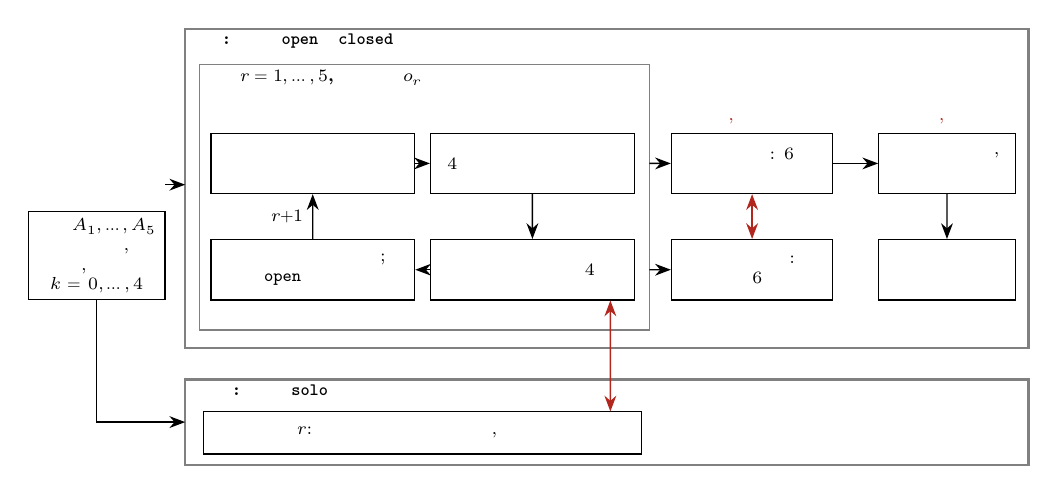
\begin{tikzpicture}[scale=.9,transform shape,
  st/.style={draw,rectangle,align=center,font=\scriptsize,inner sep=2.5pt,minimum height=.85cm,line width=.5pt,fill=white},
  fr/.style={draw,rectangle,line width=.5pt,gray},
  ttl/.style={font=\scriptsize\bfseries,anchor=north west,inner sep=2pt},
  tag/.style={text=acc,font=\scriptsize}]
  % внешние рамки
  \draw[fr,line width=.8pt] (2.2,0.2) rectangle (14.1,-4.3);
  \node[ttl] at (2.25,.2) {Группа: условия \texttt{open} и \texttt{closed}};
  \draw[fr] (2.4,-.3) rectangle (8.75,-4.05);
  \node[ttl] at (2.45,-.3) {Раунд $r=1,\dots,5$, организатор $o_r$};
  % раунд
  \node[st,text width=2.7cm] (a) at (4,-1.7) {организатор раздаёт роли из меню и задания};
  \node[st,text width=2.7cm] (b) at (7.1,-1.7) {4 исполнителя отвечают только ему};
  \node[st,text width=2.7cm] (c) at (7.1,-3.2) {организатор даёт прогноз на 4 шага};
  \node[st,text width=2.7cm] (d) at (4,-3.2) {всем сообщают прогноз и факт; в \texttt{open} ещё роли всех};
  \draw[arr] (a)--(b); \draw[arr] (b)--(c); \draw[arr] (c)--(d);
  \draw[arr] (d)--node[left,font=\scriptsize,align=right] {$r{+}1$} (a);
  % голосование и судья
  \node[st,text width=2.1cm] (v1) at (10.2,-1.7) {голос цифрой: 6 пар у каждого агента};
  \node[st,text width=2.1cm] (q) at (10.2,-3.2) {голос с причиной: те же 6 пар};
  \node[st,text width=1.75cm] (v2) at (12.95,-1.7) {большинство по парам, порядок группы};
  \node[st,text width=1.75cm] (j) at (12.95,-3.2) {судья оценивает роли и ответы};
  \draw[arr] (8.75,-1.7)--(v1);
  \draw[arr] (8.75,-3.2)--(q);
  \draw[arr] (v1)--(v2);
  \draw[arr] (v2)--(j);
  % соло
  \draw[fr,line width=.8pt] (2.2,-4.75) rectangle (14.1,-5.95);
  \node[ttl] at (2.25,-4.75) {Одиночки: условие \texttt{solo}};
  \node[st,text width=6cm,minimum height=.6cm] (s) at (5.55,-5.5) {раунд $r$: агент один прогнозирует то же окно, видит свой итог};
  \node[font=\scriptsize,anchor=west] at (9,-5.5) {Голосования и судьи нет};
  % вход
  \node[st,text width=1.75cm] (in) at (.95,-3) {агенты $A_1,\dots,A_5$ одной модели, ряд, повторы $k=0,\dots,4$};
  \draw[arr] (in.east|-0,-2) -- (2.2,-2);
  \draw[arr] (in.south) |- (2.2,-5.35);
  % величины
  \node[tag,anchor=south west,inner xsep=0pt] at (a.north west) {повторы ролей и составов};
  \node[tag,anchor=north] at (c.south) {ошибка прогноза};
  \draw[acc,{Stealth[length=2mm]}-{Stealth[length=2mm]},line width=.6pt] ([xshift=1.1cm]c.south)--(8.2,-5.2);
  \node[tag,anchor=west] at (8.25,-4.5) {разность ошибок одиночки и группы};
  \node[tag,anchor=south,align=center,text width=2.6cm] at (v1.north) {взаимность, связь с точностью};
  \node[tag,anchor=south,align=center,text width=2.1cm] at (v2.north) {порядок, согласие};
  \node[tag,anchor=north] at (j.south) {согласие с судьёй};
  \draw[acc,{Stealth[length=2mm]}-{Stealth[length=2mm]},line width=.6pt] (v1.south)--(q.north);
  \node[tag,anchor=west] at (10.25,-2.45) {расхождение};
\end{tikzpicture}

\vspace{1mm}
\raggedright\scriptsize Голос цифрой и голос с причиной агент даёт по одной и той же истории, и ни один из этих ответов в неё не попадает. Здесь $r$ --- номер раунда, $k$ --- номер повтора, $o_r$ --- организатор раунда $r$, равный $A_{((r+k-1)\bmod 5)+1}$, а окно --- четыре шага ряда, которые прогнозируются в раунде. Рамка запуска повторяется для каждого условия и каждого $k$; в \texttt{solo} порядок агентов и окна те же. Красным показаны измеряемые величины.
\end{frame}

\begin{frame}{Схема эксперимента}
\centering
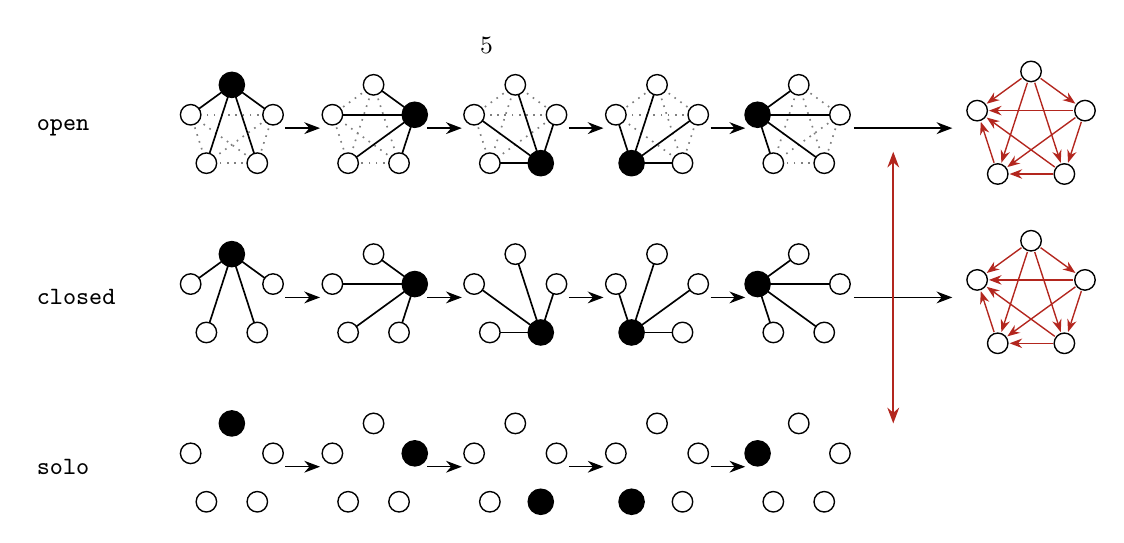
\begin{tikzpicture}[
  ag0/.style={draw,circle,fill=white,minimum size=2.6mm,inner sep=0pt,line width=.5pt},
  ag1/.style={draw,circle,fill=black,minimum size=3.2mm,inner sep=0pt,line width=.5pt},
  lbl/.style={font=\small\ttfamily,anchor=west}]
  \node[font=\small] at (6.2,1.05) {5 раундов};
  \node[font=\small] at (12.75,1.05) {голосование};
  \foreach \y/\m/\t in {0/2/open,-2.15/1/closed,-4.3/0/solo}{
    \node[lbl] at (0,\y) {\t};
    \foreach \r in {1,...,5}{
      \pgfmathsetmacro{\x}{2.6+(\r-1)*1.8}
      \glyph{\x}{\y}{\r}{\m}
      \ifnum\r<5 \draw[arr] ({\x+.68},\y)--({\x+1.12},\y);\fi
    }
  }
  \foreach \y in {0,-2.15}{\draw[arr] (10.5,\y)--(11.75,\y); \vote{12.75}{\y}}
  \draw[{Stealth[length=2mm]}-{Stealth[length=2mm]},acc,line width=.6pt] (11,-3.75)--(11,-.3);
  \node[text=acc,font=\small,anchor=west] at (11.05,-4.3) {точность};
\end{tikzpicture}

\vspace{1mm}
\scriptsize Чёрный --- организатор раунда; линии --- задания и ответы; пунктир --- роли видны всем; стрелки --- победы в парах.
\end{frame}

\begin{frame}{Что агент знает в момент голосования}
\vspace{-2mm}
\centering
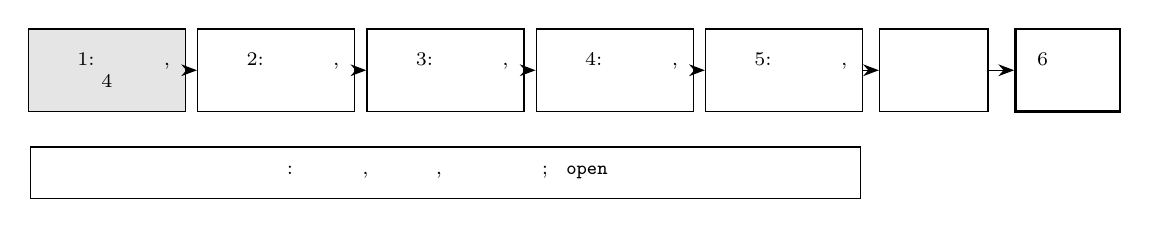
\begin{tikzpicture}[
  st/.style={draw,rectangle,align=center,font=\scriptsize,inner sep=2.5pt,minimum height=1.05cm,line width=.5pt,text width=1.82cm}]
  \node[st,fill=black!10] (r1) at (1,0) {раунд 1: \textbf{организатор}, читает 4 ответа};
  \foreach \i/\x in {2/3.15,3/5.3,4/7.45,5/9.6}
    \node[st] (r\i) at (\x,0) {раунд \i: исполнитель, своя роль и свой ответ};
  \foreach \a/\b in {1/2,2/3,3/4,4/5} \draw[arr] (r\a)--(r\b);
  \node[draw,align=center,font=\scriptsize,line width=.5pt,minimum height=.65cm,text width=10.3cm] (sum) at (5.3,-1.3) {после каждого раунда всем: организатор, его прогноз, реальные значения; в \texttt{open} ещё роли и задания всех};
  \node[st,text width=1.2cm] (d) at (11.5,0) {итог для себя};
  \node[st,text width=1.15cm,line width=.9pt] (v) at (13.2,0) {6 вопросов о парах};
  \draw[arr] (r5)--(d); \draw[arr] (d)--(v);
\end{tikzpicture}

\vspace{2mm}
\raggedright
\begin{columns}[T]
\begin{column}{.5\textwidth}
\footnotesize Показан агент, организующий раунд 1; у остальных агентов серым выделен другой раунд.

\smallskip
\textbf{В памяти есть}

\smallskip
прогноз каждого организатора и факт, поэтому точность агент может вычислить сам;

\smallskip
роль и ответ агента в каждом раунде, а также 4 ответа в раунде, который он вёл;

\smallskip
сообщение, что работу оценивают внешние эксперты.
\end{column}
\begin{column}{.46\textwidth}
\footnotesize\textbf{В памяти нет}

\smallskip
ответов исполнителей в чужих раундах;

\smallskip
чужих ролей в \texttt{closed}, кроме розданных им самим;

\smallskip
готовых значений ошибки и оценок судьи;

\smallskip
предупреждения о голосовании до самого вопроса.
\end{column}
\end{columns}
\end{frame}

\begin{frame}{Вопросы о ролях и точности}
\footnotesize
\renewcommand{\arraystretch}{1.5}
\begin{tabular}{@{}p{4.1cm}p{9.3cm}@{}}
\toprule
Вопрос & Величина и уровень сравнения\\
\midrule
\textbf{Закрепляются ли роли за агентами?} & $F$ --- сколько раз агент снова получил прежнюю роль; сравниваем со случайной раздачей тех же ролей\\
\textbf{Передаётся ли состав ролей?} & $C$ --- сколько раз набор ролей раунда совпал с набором предыдущего; сравниваем с независимым выбором наборов\\
\textbf{Точнее ли группа одиночки?} & $\mathrm{MASE}$ --- ошибка прогноза, делённая на ошибку прогноза «как на прошлой неделе»; $\Delta Q$ --- $\mathrm{MASE}$ одиночки минус $\mathrm{MASE}$ группы на том же окне\\
\bottomrule
\end{tabular}

\bigskip
Здесь $p$ --- вероятность при нулевой гипотезе получить значение не меньше наблюдаемого. Формулы --- в запасных слайдах.
\end{frame}

\begin{frame}{Вопросы о голосовании}
\scriptsize
\renewcommand{\arraystretch}{1.3}
\begin{tabular}{@{}p{4.1cm}p{9.3cm}@{}}
\toprule
Вопрос & Величина и уровень сравнения\\
\midrule
\textbf{Складываются ли голоса в порядок без циклов?} & $h$ --- доля троек агентов без цикла в итоге попарного большинства; сравниваем со случайными голосующими\\
\textbf{Согласны ли агенты, кто должен руководить?} & $U$ --- среднее по запускам число пар кандидатов, которые трое голосующих решили одинаково; сравниваем со случайными голосующими. $L$ --- число запусков, где лидирует самый частый лидер; сравниваем со сменой имён агентов\\
\textbf{Взаимны ли предпочтения?} & $\tau^{\mathrm{rec}}$ --- согласие мест, которые два агента дают друг другу; сравниваем с одними общими предпочтениями\\
\textbf{Выбирают ли агенты самых точных организаторов?} & $\tau^{\mathrm{acc}}$ --- согласие порядка голосующего с порядком агентов по ошибке; $H$ --- сколько голосующих поставили первым самого точного; сравниваем с перемешанными ошибками\\
\textbf{Совпадает ли выбор агентов с оценкой судьи?} & $\tau^{\mathrm J}$ --- согласие порядка голосующего с порядком организаторов по оценке судьи за распределение ролей; сравниваем с перемешанными оценками\\
\bottomrule
\end{tabular}

\medskip
Здесь $\tau$ --- коэффициент Кендалла между двумя порядками.
\end{frame}

\begin{frame}{Результаты: роли и точность}
\small
\textbf{Если назначения видны всем, агент обычно снова получает прежнюю роль.} Из 75 возможных случаев так происходит 67, 64 и 69 раз в \texttt{open} и 28, 39 и 33 раза в \texttt{closed} (старшая Gemma, Qwen, YandexGPT), тогда как случайная раздача тех же ролей даёт от 12 до 17 раз. На младшей Gemma получено 33 из 45 в \texttt{open} и 9 из 30 в \texttt{closed}, на DeepSeek 12 из 15 в \texttt{open}.

\medskip
\textbf{Организаторы не перенимают набор ролей друг у друга.} Набор совпадает с предыдущим не чаще, чем при независимом выборе: наименьшее $p$ по всем запускам равно $0{,}077$.

\medskip
\textbf{Группа прогнозирует не точнее одиночки.} На одном и том же окне группа точнее в 23 случаях из 50 на старшей Gemma ($p=0{,}67$), в 22 из 50 на YandexGPT ($p=0{,}77$) и в 11 из 25 на младшей Gemma ($p=0{,}69$). На Qwen она точнее только в 17 случаях из 50 ($p=0{,}044$).
\end{frame}

\begin{frame}{Результаты: голосование}
\footnotesize
\textbf{Отсутствие циклов не отличает агентов от случайных голосующих.} На полных сериях $h$ лежит от $0{,}40$ до $1{,}00$, а у случайных голосующих 95\% значений лежат от $0{,}60$ до $1{,}00$, поэтому при пяти агентах этот показатель почти ничего не различает.

\smallskip
\textbf{Внутри запуска агенты чаще случайного выбирают одного и того же кандидата.} Каждую из 10 пар кандидатов решают трое остальных агентов. Все трое выбирают одного кандидата в среднем в 4{,}4, 5{,}2 и 5{,}8 парах в \texttt{open} ($p\le 0{,}006$) и в 2{,}4, 3{,}8 и 4{,}0 парах в \texttt{closed} ($p=0{,}60$, $0{,}042$ и $0{,}024$), тогда как случайные голосующие дают 2{,}5 пары (порядок серий: старшая Gemma, Qwen, YandexGPT).

\smallskip
\textbf{Лидер от запуска к запуску обычно меняется.} Исключение одно: на YandexGPT в \texttt{open} агент $A_3$ лидирует в 4 запусках из 5 ($p=0{,}006$).

\smallskip
\textbf{Взаимность объясняется общими предпочтениями.} Выше их уровня $\tau^{\mathrm{rec}}$ поднимается только на старшей Gemma в \texttt{open} ($+0{,}31$ против $+0{,}13$), но превышение держится на одном запуске: без него $p=0{,}145$.

\smallskip
\textbf{Агенты не выбирают самых точных организаторов.} Самого точного организатора ставят первым 12, 13 и 11 голосующих из 50 при 12{,}5 у случайных; наименьшее $p$ по условиям равно $0{,}266$, а с поправкой на трудность окна $0{,}074$.

\smallskip
\textbf{Выбор агентов не связан с оценкой судьи.} Средняя $\tau^{\mathrm J}$ в \texttt{open} и \texttt{closed} равна $-0{,}01$ и $+0{,}01$ на старшей Gemma, $+0{,}07$ и $+0{,}17$ на Qwen, причём все $p\ge 0{,}299$. На YandexGPT судьёй была та же модель, и оценки различались лишь в 2 запусках из 10, поэтому вывода по ней нет.
\end{frame}

\begin{frame}{Итог}
\footnotesize
\renewcommand{\arraystretch}{1.25}
\begin{tabular}{@{}ll@{}}
\toprule
Вопрос & Ответ\\
\midrule
Закрепляются ли роли? & да, и сильнее при видимых назначениях\\
Передаётся ли состав ролей? & нет\\
Точнее ли группа одиночки? & нет; на Qwen группа хуже на границе значимости\\
Есть ли порядок без циклов? & не отличим от случайного, тест слабый\\
Согласны ли агенты о руководителе? & в запуске да, между повторами почти нет\\
Взаимны ли предпочтения? & объясняются общими предпочтениями\\
Выбирают ли самых точных организаторов? & нет\\
Совпадает ли выбор с оценкой судьи? & нет; по YandexGPT вывода нет\\
\bottomrule
\end{tabular}

\bigskip
\footnotesize\textbf{Ограничения.} На условие приходится пять повторов на одном временном ряду, поэтому слабые эффекты не обнаруживаются. Серии различаются моделью, а часть и языком промптов, так что напрямую мы их не сравниваем. Выводы о голосовании не распространяются на младшую Gemma, поскольку её голос отражает место кандидата в паре. Меню ролей и очерёдность организаторов заданы экспериментатором.
\end{frame}

\begin{frame}{Какие условия можно добавить}
\scriptsize
\renewcommand{\arraystretch}{1.0}\setlength{\tabcolsep}{4pt}\hyphenpenalty=10000
\begin{tabular}{@{}p{6.5cm}p{7cm}@{}}
\toprule
Что меняем & Что узнаем\\
\midrule
\multicolumn{2}{@{}l}{\textbf{Зачем нужно закрепление ролей}}\\
Виден набор ролей, но не видно, кому какая досталась & Если закрепление исчезнет, оно держалось на том, кто какую роль получал\\
Роли раздаёт среда: за агентом постоянно или заново в каждом раунде & Если постоянные роли дают меньшую ошибку, закрепление полезно для прогноза\\
Организатор опрашивает агентов без ролей & Если ошибка та же, роли ничего не добавляют\\
\midrule
\multicolumn{2}{@{}l}{\textbf{Откуда берутся закрепление и согласие}}\\
Агент не помнит прошлых раундов, кроме их итогов & Если закрепление в \texttt{closed} исчезнет, оно шло от памяти агента\\
Перед голосованием агент не пишет итог для себя & Если голоса изменятся, этот итог влияет на выбор\\
Перед голосованием скрыты прогнозы и реальные значения & Если согласие сохранится, оно не опирается на итоги раундов\\
\midrule
\multicolumn{2}{@{}l}{\textbf{Что будет при большей свободе и разных агентах}}\\
Следующего организатора выбирают голосованием & Появится ли устойчивый лидер, когда выбор влияет на работу\\
Агенты видят разные данные & Выберет ли группа агента с лучшими данными\\
Агенты пишут друг другу напрямую & Станет ли группа точнее одиночки без посредника\\
\bottomrule
\end{tabular}

\smallskip
Выбор организатора голосованием нарушает очерёдность, так что с нынешними сериями по $\Delta Q$ его сравнить нельзя.
\end{frame}

\begin{frame}
\centering\Large Запасные слайды
\end{frame}

\begin{frame}{Один раунд в группе}
\begin{columns}[T]
\begin{column}{.46\textwidth}
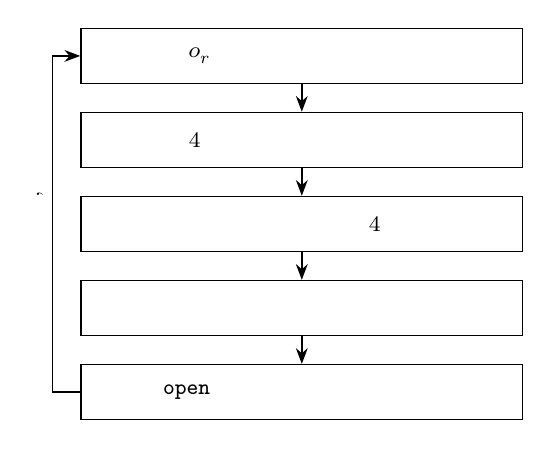
\begin{tikzpicture}[node distance=3.5mm]
  \tikzset{b/.style={box,text width=5.4cm,minimum height=.7cm}}
  \node[b] (a) {организатор $o_r$ выбирает каждому исполнителю роль и задание};
  \node[b,below=of a] (b) {4 исполнителя отвечают организатору};
  \node[b,below=of b] (c) {организатор даёт прогноз на 4 шага};
  \node[b,below=of c] (d) {всем агентам сообщают прогноз и реальные значения};
  \node[b,below=of d] (e) {в \texttt{open} им также сообщают роли и задания всех};
  \foreach \x/\y in {a/b,b/c,c/d,d/e} \draw[arr] (\x)--(\y);
  \draw[arr] (e.west)--++(-.35,0)|-(a.west);
  \node[rotate=90,font=\scriptsize,anchor=south] at ($(b.west)!.5!(c.west)+(-.35,0)$) {следующий раунд, другой организатор};
\end{tikzpicture}
\end{column}
\begin{column}{.52\textwidth}
\scriptsize
\textbf{Что видит агент}

\smallskip
\begin{tabular}{@{}lccc@{}}
\toprule
 & \texttt{open} & \texttt{closed} & \texttt{solo}\\
\midrule
своя роль и задание & да & да & ---\\
роли и задания всех & да & нет & ---\\
ответы исполнителей & \multicolumn{2}{c}{организатор} & ---\\
прогноз и факт & все & все & свои\\
\bottomrule
\end{tabular}

\bigskip
\textbf{Меню ролей}

\smallskip
Историк, календарь, моделист, статистик, сценарист, критик. Организатор может дать одну роль нескольким исполнителям и не использовать часть ролей, но не может ввести новую.
\end{column}
\end{columns}
\end{frame}

\begin{frame}{Голосование}
\begin{columns}[T]
\begin{column}{.36\textwidth}
\centering
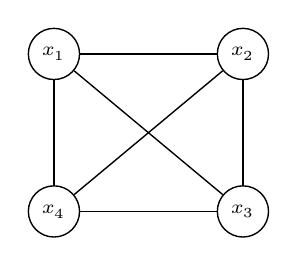
\begin{tikzpicture}
  \node[ag] (a) at (0,2) {$x_1$}; \node[ag] (b) at (2.4,2) {$x_2$};
  \node[ag] (c) at (2.4,0) {$x_3$}; \node[ag] (d) at (0,0) {$x_4$};
  \foreach \p/\q in {a/b,a/c,a/d,b/c,b/d,c/d} \draw[line width=.5pt] (\p)--(\q);
\end{tikzpicture}

\medskip
\footnotesize Голосующий $v$ отвечает на 6 вопросов: по одному на каждое ребро графа $K_4$, вершины которого $x_1,\dots,x_4$ --- остальные агенты.
\end{column}
\begin{column}{.6\textwidth}
\footnotesize
\textbf{Вопрос.} Кого из двух кандидатов назначить организатором прогноза на 13 шагов, по ходу которого проверок не будет? Голоса тайные, вопросы задаются от одного состояния памяти и в историю не попадают.

\medskip
\textbf{Голос цифрой.} Агент отвечает одной цифрой. Пусть $P_v(x\mid\{x,y\})$ --- вероятность, с которой $v$ в паре кандидатов $\{x,y\}$ называет цифру кандидата $x$. Предпочтение равно
\[m_v(x,y)=\log P_v(x\mid\{x,y\})-\log P_v(y\mid\{x,y\}).\]

\textbf{Итог.} Кандидат выигрывает пару, если за него больше голосов из трёх остальных агентов. Агенты упорядочены по числу выигранных пар.

\medskip
\textbf{Голос с причиной.} Параллельно голосу цифрой те же пары задаются от той же истории агента. Ответ содержит выбор и причину. Отдельная проба задаёт одному агенту каждую его пару 5 раз.
\end{column}
\end{columns}
\end{frame}

\begin{frame}{Обозначения}
\small
Положим $\mathcal A=\{A_1,\dots,A_5\}$, а $\mathcal R$ --- меню из шести ролей. Раунд $r$ организует $o_r$, исполнители образуют множество $\mathcal W_r=\mathcal A\setminus\{o_r\}$, а $\rho_r(i)\in\mathcal R$ --- роль исполнителя $i$.

\medskip
Для голосующего $v$ и кандидата $x\ne v$ суммарный перевес равен
\[s_v(x)=\sum_{y\notin\{v,x\}}m_v(x,y),\]
а $\pi_v(x)\in\{1,\dots,4\}$ --- место $x$ в порядке убывания $s_v$.

\medskip
Пусть $a(x)$ и $b(x)$ --- места элемента $x$ в двух порядках на множестве $S$. Коэффициент Кендалла равен
\[\tau(a,b)=\binom{\lvert S\rvert}{2}^{-1}\sum_{\{x,y\}\subset S}\sgn\bigl(a(x)-a(y)\bigr)\sgn\bigl(b(x)-b(y)\bigr).\]

Пусть $T$ --- наблюдаемая статистика, а $T^\ast$ --- её значение в одном из $M$ розыгрышей нулевой гипотезы. Тогда $p=\dfrac{1+\#\{T^\ast\ge T\}}{M+1}$. Символ $\ind[\cdot]$ обозначает индикатор, а единица анализа --- запуск.
\end{frame}

\begin{frame}{Закрепление ролей $F$}
\small Пусть $\mathrm{prev}_r(i)$ --- предыдущий раунд, в котором агент $i$ был исполнителем. Число повторов равно
\[F=\sum_{r}\ \sum_{\substack{i\in\mathcal W_r\\ \mathrm{prev}_r(i)\text{ определён}}}\ind\bigl[\rho_r(i)=\rho_{\mathrm{prev}_r(i)}(i)\bigr],\qquad 0\le F\le 15.\]

\textbf{Нулевая гипотеза.} В каждом раунде набор ролей $\{\rho_r(i)\}_{i\in\mathcal W_r}$ сохраняется и независимо переставляется между теми же исполнителями. Значение $p$ одностороннее, $M=20000$.

\medskip
Эта гипотеза учитывает выбор ролей организаторами, поэтому $F$ сверх него измеряет привязку роли к конкретному агенту.

\medskip
\textbf{Специализация} агента $i$ равна доле его назначений на самую частую роль:
\[\mathrm{sp}(i)=\max_{q\in\mathcal R}\frac{\#\{r:\rho_r(i)=q\}}{\#\{r:i\in\mathcal W_r\}}.\]
\end{frame}

\begin{frame}{Повтор состава ролей $C$}
\small Состав раунда --- множество ролей без учёта кратности и исполнителей: $S_r=\{\rho_r(i):i\in\mathcal W_r\}\subseteq\mathcal R$. Число повторов при смене организатора равно
\[C=\sum_{r=2}^{5}\ind[S_r=S_{r-1}],\qquad 0\le C\le 4.\]

\textbf{Нулевая гипотеза.} Составы $S_1^\ast,\dots,S_5^\ast$ независимо выбираются из эмпирического набора составов всех запусков того же условия и серии. Так повторы от общего предпочтения одного состава не считаются передачей схемы.

\medskip
Пусть $C^\ast$ --- значение $C$ в розыгрыше, а $\mathbb E C^\ast$ --- его среднее по розыгрышам. Значение $p$ двустороннее, $M=20000$:
\[p=\frac{1+\#\{\lvert C^\ast-\mathbb E C^\ast\rvert\ge\lvert C-\mathbb E C^\ast\rvert\}}{M+1}.\]
\end{frame}

\begin{frame}{Ошибка прогноза $\MASE$}
\small Пусть $y_t$ --- значение ряда на шаге $t$, а $t_r=52+4(r-1)$. В раунде $r$ агент видит историю $y_{t_r-51},\dots,y_{t_r}$ и даёт прогноз $\hat y_{t_r+1},\dots,\hat y_{t_r+4}$. Ошибка нормируется на ошибку наивного прогноза $\hat y_{t+1}=y_t$ на видимой истории:
\[\MASE_r=\frac{\dfrac14\displaystyle\sum_{j=1}^{4}\bigl\lvert\hat y_{t_r+j}-y_{t_r+j}\bigr\rvert}{\dfrac1{51}\displaystyle\sum_{s=t_r-50}^{t_r}\lvert y_s-y_{s-1}\rvert}.\]

При $\MASE_r<1$ прогноз точнее наивного на истории. Знаменатель зависит только от окна, поэтому внутри одного окна сравнение зависит только от числителя.

\medskip
Эта величина зависит от трудности окна, поэтому условия сравниваются по $\Delta Q$.
\end{frame}

\begin{frame}{Коллективный выигрыш $\Delta Q$}
\small Пусть $\MASE^{c}_{k,r}$ --- ошибка условия $c$ в повторе $k$ и раунде $r$. Для $c\in\{\texttt{open},\texttt{closed}\}$ положим
\[\Delta Q_{c,k,r}=\MASE^{\texttt{solo}}_{k,r}-\MASE^{c}_{k,r}.\]
В этом сравнении совпадают окно и агент, ведущий раунд. При $\Delta Q>0$ группа точнее.

\medskip
\textbf{Проверка.} Пусть из $n$ ненулевых разностей положительны $n_+$. Тест точный, знаковый и двусторонний:
\[p=\min\Bigl(1,\ 2\cdot 2^{-n}\sum_{i=0}^{\min(n_+,\,n-n_+)}\binom ni\Bigr).\]
Пары внутри запуска зависимы, поэтому $p$ --- ориентировочная оценка.

\medskip
\textbf{Независимый ансамбль.} Пусть $\hat y^{\,c}_{k,r,t}$ --- прогноз условия $c$ в повторе $k$ и раунде $r$ на шаг $t$. На каждом шаге берётся медиана по повторам, и по ней считается $\MASE$:
\[\hat y^{\,\med,c}_{r,t}=\med_{k}\hat y^{\,c}_{k,r,t},\qquad c\in\{\texttt{open},\texttt{closed},\texttt{solo}\}.\]
\end{frame}

\begin{frame}{Линейность порядка $h$}
\small Кандидат $x$ выигрывает пару $\{x,y\}$, если среди трёх голосующих $v\notin\{x,y\}$ больше тех, у кого $m_v(x,y)>0$. Обозначим через $w(x)$ число пар, выигранных агентом $x$. Индекс Ландау равен
\[h=\binom{5}{3}^{-1}\sum_{x\in\mathcal A}\binom{w(x)}{2}.\]

При полном порядке без циклов $h=1$, а каждая циклическая тройка уменьшает сумму. Пары без большинства не дают побед и тоже уменьшают $h$.

\medskip
\textbf{Нулевая гипотеза.} Предпочтения каждого голосующего --- независимый равномерно случайный порядок; из $M=20000$ розыгрышей берутся среднее и 95\%-интервал.

\medskip
\textbf{Сопутствующие величины}: медиана $\lvert m_v(x,y)\rvert$, число единодушных пар (3:0) и доля транзитивных троек у отдельного голосующего.
\end{frame}

\begin{frame}{Согласие о руководителе $U$ и $L$}
\small Пара единодушна, если все три голосующих решили её одинаково. Для запуска $k$ положим
\[U_k=\sum_{\{x,y\}\subset\mathcal A}\ind\bigl[\sgn m_v(x,y)\text{ одинаков при всех }v\notin\{x,y\},\ m_v(x,y)\ne 0\bigr],\qquad 0\le U_k\le 10,\]
а $U$ --- среднее $U_k$ по запускам условия.

\textbf{Нулевая гипотеза для $U$.} Предпочтения голосующих --- независимые равномерно случайные порядки, поэтому $\mathbb E U_k=10/4$. Значение $p$ одностороннее, $M=20000$.

\medskip
Пусть $\Lambda_k$ --- агенты с наибольшим числом побед в запуске $k$. Лидер получает долю $1/\lvert\Lambda_k\rvert$, поэтому равенство побед не решается именем агента. Сумма долей самого частого лидера равна
\[L=\max_{a\in\mathcal A}\sum_{k}\frac{\ind[a\in\Lambda_k]}{\lvert\Lambda_k\rvert}.\]

\textbf{Нулевая гипотеза для $L$.} Имена агентов независимо переставляются внутри каждого запуска. Значение $p$ одностороннее, $M=20000$.
\end{frame}

\begin{frame}{Взаимность $\tau^{\mathrm{rec}}$}
\small Каждой паре агентов $\{i,j\}$ сопоставим точку $\bigl(\pi_i(j),\pi_j(i)\bigr)$. По 10 точкам считается
\[\tau^{\mathrm{rec}}=\binom{10}{2}^{-1}(\#\text{согласных пар точек}-\#\text{несогласных пар точек}),\]
причём пары точек с равной координатой не входят в разность.

\medskip
\textbf{Первая нулевая гипотеза.} Порядки голосующих независимы и равномерно случайны.

\medskip
\textbf{Вторая нулевая гипотеза: общие предпочтения.} Оценка раскладывается на популярность кандидата и остаток:
\[s_v(x)=\bar s(x)+\varepsilon_v(x),\qquad \bar s(x)=\frac14\sum_{v\ne x}s_v(x),\]
где $\bar s(x)$ --- популярность, а $\varepsilon_v(x)$ --- остаток.
Остатки перемешиваются по всем парам $(v,x)$, что сохраняет популярность и разброс, но разрушает связь внутри пар. Общие предпочтения сами дают $\tau^{\mathrm{rec}}>0$, поэтому одностороннее $p$ считается против этой гипотезы, $M=2000$.
\end{frame}

\begin{frame}{Связь выбора с точностью $\tau^{\mathrm{acc}}$}
\small Пусть $r(x)$ --- раунд, который организовал агент $x$. Его ошибка равна $e(x)=\MASE_{r(x)}$. С поправкой на трудность окна из неё вычитается среднее значение $\MASE$ того же окна по запускам условия.

\medskip
Пусть $E_v$ --- порядок агентов $\mathcal A\setminus\{v\}$ по возрастанию $e$. Тогда
\[\tau^{\mathrm{acc}}=\frac15\sum_{v\in\mathcal A}\tau(\pi_v,E_v),\qquad H=\sum_{v\in\mathcal A}\ind\Bigl[\pi_v^{-1}(1)=\arg\min_{x\ne v}e(x)\Bigr].\]

$H$ --- число голосующих, поставивших первым самого точного; случайный уровень для него равен $1/4$ на голосующего. Отдельно считается, совпал ли победитель голосования с самым точным организатором (случайный уровень $1/5$ на запуск).

\medskip
\textbf{Нулевая гипотеза.} Ошибки перемешиваются между агентами внутри запуска, поскольку голоса внутри запуска зависимы. Значения $p$ односторонние, $M=2000$.
\end{frame}

\begin{frame}{Согласие с судьёй $\tau^{\mathrm J}$}
\small Судья работает после голосования в отдельных запросах. Он не знает, кто был организатором, и не видит реальных значений, а агентам его оценки не передаются. Всего в запуске 25 запросов.

\medskip
\begin{tabular}{@{}lll@{}}
\toprule
Шкала от 1 до 5 & Что оценивает & Число оценок\\
\midrule
\texttt{allocation} & распределение ролей организатором & 5\\
\texttt{role\_fit} & соответствие ответа роли и заданию & 20\\
\texttt{usefulness} & польза ответа для прогноза & 20\\
\bottomrule
\end{tabular}

\bigskip
Пусть $J_v$ --- порядок организаторов $\mathcal A\setminus\{v\}$ по убыванию \texttt{allocation}. Тогда
\[\tau^{\mathrm J}_v=\tau(\pi_v,J_v).\]
Для группы так же сравнивается порядок по числу побед $w(x)$, введённому на слайде о порядке голосов. Если все оценки запуска равны, порядка нет и значение не определено. По условию $\tau^{\mathrm J}_v$ усредняется, а нулевая гипотеза перемешивает оценки между агентами внутри запуска; $p$ одностороннее, $M=2000$.
\end{frame}

\begin{frame}{Влияние вопроса о причине $\varphi$}
\small Голос с причиной даёт для голосующего $v$ и пары $\{x,y\}$ выбор $c_v(x,y)\in\{x,y\}$. Пусть $\mathcal P$ --- множество упорядоченных так троек $(v,x,y)$, что перевес голоса цифрой $m_v(x,y)>0$. Доля изменившихся пар равна
\[\varphi=\frac{1}{\lvert\mathcal P\rvert}\sum_{(v,x,y)\in\mathcal P}\ind\bigl[c_v(x,y)=y\bigr].\]

Порядок голосующего в голосе с причиной $\pi'_v$ строится по числу выборов, а при равенстве --- по сумме перевесов. Сходство с голосом цифрой равно $\tau(\pi_v,\pi'_v)$.

\medskip
\textbf{Устойчивость.} В пробе с пятью вызовами на пару совпадение всех пяти выборов сравнивается с $\lvert m_v(x,y)\rvert$. Причина пишется после выбора, поэтому мотивом выбора не считается.
\end{frame}

\end{document}
